\chapter{Literature Review}\label{chap:lit}

\section{Fairness in Algorithmic Decision Making}\label{sec:fairness}

Due to the increasing use of decision-making algorithms for varying applications, the topic of \textit{Fairness} has become a heavily researched topic in the field of Machine Learning and AI.\@
While fairness concerns do not take an important role in all kinds of algorithmic decision making (some algorithms simply do not have grave enough implications to make fairness a concern, an example being buying recommendation algorithms \parencite{Marcinkevics2023}), 
they need to be focused on in applications like hiring processes or criminal justice systems, where the decisions could heavily impact individuals \parencite{Barocas2016}.
As this thesis is based on mortgage lending data and builds upon the analysis of demographic attributes like race or gender, fairness concerns are of utmost importance and will be discussed in the following sections.

\subsection{Overview of Fairness in Algorithmic Decision Making}\label{subsec:overview}

The intensive research of Fairness in algorithmic decision making results in a wide range of definitions of Fairness as well as methods to assess it \parencite{CorbettDavies2023}.
Most of these are of \textit{mathematical} or quantitative nature, however, there also is somewhat separate approach of assessing fairness \textit{individually} in a qualitative way \parencite{Chouldechova2018}.
Before presenting the most prominent mathematical measures of fairness, it should be noted that while there are different reasons for unfairness to arise (see~\cite{Chouldechova2018} for a brief overview), bias in the underlying data (through discrimination, erroneous inputs or imbalances in the distributions) 
is the main reason for unfairness to arise \parencite{Choras2020}\footnote{The reasons for bias in the underlying data are a highly interesting area of research, but out of the scope of this thesis. See~\cite{Mehrabi2021} for an extensive list and discussion for types and reasons for biased data}.
Measuring the impact of these biases on model fairness, several approaches have gained increased attention from researchers\footnote{This selection is based on the paper by Pessach and Shmueli \parencite{Pessach2020}, who also provide a more extensive overview of measurements not as commonly used in academic literature}:
\begin{itemize}
    \item \textbf{Disparate Impact} is based on the expected positive prediction rate for each group. For a fair outcome, the rate of positive predictions for any group should be on par or just slightly below the rate for any other group. Formally: 
    \begin{equation}
    \frac{P(\hat{Y} = 1|S \neq 1)}{P(\hat{Y} = 1|S = 1)} \geq 1 - \varepsilon
    \label{eq:disparate_impact}
    \addcontentsline{frm}{formulas}{\protect\numberline{\theequation}\hspace{1em}Disparate Impact}
    \end{equation}
    where $\hat{Y} = 1$ refers to a positive prediction, $S$ is the protected attribute, $S=1$ is a potentially privileged group, $S \neq 1$ is a potentially disadvantaged group and $\varepsilon$ refers to the allowed threshold.

    \item \textbf{Statistical Parity} is similar to the measurement of Disparate Impact, but works with the difference instead of the ratio. Formally:
    \begin{equation}
    \left| P\left[\hat{Y} = 1|S = 1\right] - P\left[\hat{Y} = 1|S \neq 1\right] \right| \leq \epsilon
    \label{eq:statistical_parity}
    \addcontentsline{frm}{formulas}{\protect\numberline{\theequation}\hspace{1em}Statistical Parity}
    \end{equation}

    \item \textbf{Equalized Odds} is based on the True Positive Rate (TPR) and the False Positive Rate (FPR). For a fair outcome, both rates should be (close to) equal for all groups. Formally:
    \begin{equation}
    \left| P[\hat{Y} = 1|S = 1, Y = 0] - P[\hat{Y} = 1|S \neq 1, Y = 0] \right| \leq \epsilon
    \label{eq:equalized_odds_1}
    \addcontentsline{frm}{formulas}{\protect\numberline{\theequation}\hspace{1em}Equalized Odds (1)}
    \end{equation}
    \begin{equation}
    \left| P[\hat{Y} = 1|S = 1, Y = 1] - P[\hat{Y} = 1|S \neq 1, Y = 1] \right| \leq \epsilon
    \label{eq:equalized_odds_2}
    \addcontentsline{frm}{formulas}{\protect\numberline{\theequation}\hspace{1em}Equalized Odds (2)}
    \end{equation}
    where~\eqref{eq:equalized_odds_1} and~\eqref{eq:equalized_odds_2} restrict the difference in TPR and FPR for the two groups to be smaller than $\varepsilon$ respectively.

    \item \textbf{Equal Opportunity} is similar to Equalized Odds, but only focuses on the TPR. Formally:
    \begin{equation}
    \left| P[\hat{Y} = 1|S \neq 1, Y = 1] - P[\hat{Y} = 1|S = 1, Y = 1] \right| \leq \epsilon
    \label{eq:equal_opportunity}
    \addcontentsline{frm}{formulas}{\protect\numberline{\theequation}\hspace{1em}Equal Opportunity}
    \end{equation}
\end{itemize}

A crucial element in the Fairness discussion is the concept of \textit{protected} or \textit{sensitive attributes}. These describe attributes that are legally protected from being the basis of potentially discriminatory decisions \parencite{Datta2017}.
Protected attributes usually contain demographic information like age, race or gender (identity) \parencite{Teodorescu2020}. There are definitions available specifically for the case of mortgage lending \parencite{Chen2019}\footnote{Note that the attributes defined in the paper by Chen et al.\ apply specifically to laws of the United States of America}. 
Even though recent studies have suggested that racial bias might not be as prevalent in both human-made and algorithmic decisions as it has been assumed \parencite{Bhutta2022}, 
it is still apparent that bias-related fairness concerns are a major issue in algorithmic decision making \parencite{Mehrabi2021}.
Moreover, race is just one of the protected attributes present in the dataset analyzed in this thesis, meaning that other features present in the data can still be a source of unfairness.

\subsection{Fairness in Practice}\label{subsec:practice}

While there are a multitude of approaches to fair ML algorithms being discussed in academic literature (compare e.g.\ \cite{Mehrabi2021}), the scope of this thesis primarily includes \textit{Fair Modeling}, i.e.\ the development of fair ML algorithms, and \textit{Fairness Assessment}, i.e.\ the evaluation of the fairness of a given model

%To-Do:
%Fairness assessment (methods and metrics with formulas - aequitas, Onetto, Chouldechova, Corbett-Davies and Pessach)


\textbf{Fair Modeling} \newline
Fair Modeling is the process of developing fair ML algorithms. This can be done in three different stages: \textit{Pre-processing}, \textit{In-processing} and \textit{Post-processing} \parencite{Pessach2020}. \newline
\textit{Pre-Processing} focuses on modifying the training data in a way that removes potential biases in order to have the model learn from unbiased data \parencite{Bellamy2019}.
Several methods have been proposed in academic literature, among them \textit{massaging}, \textit{reweighing} and \textit{sampling} \parencite{Kamiran2012}, editing features and labels of the underlying dataset following fairness criteria based on a probabilistic framework \parencite{Calmon2017}, or attempts to remove disparate impact by feature value adjustment \parencite{Feldman2015}. \newline
\textit{In-Processing} aims to address unfairness during model training \parencite{Alessandro2017}. In practice, this is usually achieved by imposing constraints or adding regularization parameters to the models that explicitly aim to affect fairness criteria \parencite{Pessach2020}.
Practical examples from the academic literature include the \textit{prejudice remover regularizer} introduced by Kamishima et al. \parencite{Kamishima2012}, which is a regularizer that aims to enforce independence of predictions from protected attributes, or a method of imposing both accuracy and fairness constraints to tackle disparate impact proposed by Zafar et al. \parencite{Zafar2017}. \newline
\textit{Post-Processing} can be applied after the model training is finished. It does however rely on the availability of previously unseen holdout data \parencite{Alessandro2017}. Nevertheless, it is the only viable option if neither the underlying data nor the model itself can be modified \parencite{Bellamy2019}.
Increased Fairness through post-processing can e.g.\ be achieved by selecting different thresholds for different demographic groups or learning different classifiers for each demographic group \parencite{Pessach2020}.
A practical implementation of this approach is the work of Hardt et al.\ \parencite{Hardt2016}, where a post-processing algorithm is proposed that aims to adjust the model's predictions to achieve equalized odds (i.e.\ equal True Positive Rates and False Positive Rates for all demographic groups) while trying to improve accuracy at the same time, relying on complete information on labels, predictions and protected attributes. 

The increasing importance of Fairness considerations in Machine Learning has also led to an increased availability of tools and libraries to implement fair ML algorithms.
Two of the most prominent libraries are \textit{Aequitas}\footnote{https://github.com/dssg/aequitas} and \textit{AI Fairness 360 (AIF360)}\footnote{https://github.com/Trusted-AI/AIF360}.
Both of these libraries offer a range of features from the fair modeling and Fairness assessment steps mentioned above.

A concrete approach on how to implement fair ML algorithms in organizations and monitor their performance is proposed by Teodorescu et al.\ \parencite{Teodorescu2020}:
The proposed framework has three phases: \textit{Design}, \textit{Development} and \textit{Post-hoc Model Assessment}. Based on the presence and relevance of protected attributes (see \autoref{subsec:overview}), the authors propose different decision steps to rule out potential unfairness in the algorithm implementation.
Although being out of the scope of this thesis, this framework is a promising approach to implement fair ML algorithms in practice.

\textbf{Fairness Assessment} \newline
Fairness Assessment refers to the post-hoc evaluation of the fairness of model results. The scope of fairness can roughly be divided into the following three categories \parencite{Mehrabi2021}:
\begin{itemize}
    \item \textbf{Individual Fairness}: Individual Fairness refers to the fairness of the model's predictions for individual instances. Examples are the concept of \textit{Fairness through unawareness} \parencite{Kusner2017},  \textit{Fairness through awareness} \parencite{Dwork2012} or \textit{Fairness through counterfactuals} \parencite{Kusner2017}.
    \item \textbf{Group Fairness}: Group Fairness refers to the fairness of the model's predictions for different groups. This can be assessed by the measures introduced in \textbf{chapter \ref{subsec:overview}}.
    \item \textbf{Subgroup Fairness}: Subgroup Fairness combines the aforementioned concepts by attempting to apply group fairness measures to subsets of the underlying dataset \parencite{Kearns2019}
\end{itemize}

\subsection{Applications of Fairness in Mortgage Lending}\label{subsec:mortgage_lending_fairness}

Several studies and papers have been concerned with specifically analyzing the fairness of algorithmic decision making in the field of mortgage lending.
Nam and Yun \parencite{Nam2022} follow an approach very similar to this thesis when they used Machine Learning (specifically GANs) to infer decision rules underlying the 2018 HMDA data set in order to compare the decisions made by algorithms to man-made decisions.
Using the 2020 HMDA data set, So et al. \parencite{So2022} raise the point that indirect discrimination is present in historic loan application data and propose \textit{reparative algorithms} to tackle the issue of indirect discrimination in mortgage lending.
Their point is backed by other studies, such as the ones by Rugh et al. \parencite{Rugh2015} and Faber \parencite{Faber2013}, who prove that indirect discrimination is present in mortgage lending data and that it is a major issue in the field of Fairness in mortgage lending.
Research concerning both fairness and Explainability has been conducted by Sharma et al. \parencite{Sharma2022}, who propose a MoE model aiming to combine these two aspects as well as the ability to detect drift over time.
While this research is very promising and in some parts overlaps with the scope of this thesis, its main focus is the time component, which is not part of the scope of this thesis.

\section{Explainability and Interpretability in Machine Learning}\label{sec:Explainability}

Given the constantly increasing research into AI Interpretability and Explainability, there is surprisingly little consent on how to precisely define these concepts and how to distinguish them \parencite{Linardatos2021}. 
While both terms are used interchangeably in a multitude of publications, several studies have tried to distinguish both concepts in terms of their scope, giving rise to terms like 'xAI' (Explainable Artificial Intelligence) \parencite{Gunning2019} and occasionally also introducing related concepts like \textit{Understandability}, \textit{Comprehensibility} \parencite{Guidotti2018}, or \textit{Intelligibility} \parencite{Caruana2015}.

One of the most adapted definitions for \textit{Interpretability} has been made by Doshi-Velez and Kim, who define it as the “ability to explain or to present in understandable terms to a human” \parencite{DoshiVelez2017}. 
However, this definition does not only heavily intersect with common definitions of Explainability, it also appears to be rather general and not easily applicable in a scientific context. 
Among other unclear definitions, this has led Lipton to state that in the scientific discussion, the term Interpretability is “ill-defined”, leading to many papers in this research area only exhibiting a “quasi-scientific character” \parencite{Lipton2018}, while other authors deemed Interpretability to be a “broad, poorly defined concept” \parencite{Murdoch2019}. 
Usually, the concept of Interpretability is focused on the ability to logically comprehend the inner workings of AI algorithms, i.e.\ the user being able to predict outputs from inputs~\parencite{Kim2016}.

\textit{Explainability} or \textit{xAI} (which will be used interchangeably with the term Interpretability in this work), even though being subject to a similarly wide range of definitions, is usually defined to be more concerned with explaining the rationale behind decisions made to generate trust instead of precisely dissecting the inner workings mathematically \parencite{Gunning2019}. 
Compared to interpretable AI, which has been discussed in academic literature for a comparably longer timeframe, Explainability is a newer concept, which however seems to gather momentum in academic interest very fast, most likely due to the more and more widespread adoption of not inherently explainable Deep Learning Models \parencite{BarredoArrieta2020}.


\subsection{Inherently Interpretable Models vs. Black Box Models}\label{subsec:inherently}

Machine Learning algorithms vary in their degree of Interpretability. There usually is a trade-off between their \textit{predictive accuracy} (i.e.\ how well they perform on prediction tasks) and their \textit{descriptive accuracy} (i.e.\ how well they can be understood by humans) \parencite{Murdoch2019}, although more recent studies are challenging this assumption, compare e.g. \cite{Cooper2024}.
While some models, like linear regressions, are inherently interpretable, others, like Neural Networks, are considered to be 'black boxes' \parencite{Guidotti2018} or 'opaque models' \parencite{Burrell2016}, as their inner workings are not intuitively understandable for humans.
However, there is increased demand for models that have a high predictive accuracy while still being explainable due to, among others, legal requirements like the GDPR \parencite{GDPR} and ethical considerations \parencite{Guidotti2018}, leading to increased demand for Explainability algorithms.

\subsection{Explainability Algorithms}\label{subsec:algorithms}

This section will provide a brief overview of the different categories of Explainability algorithms, and provide additional information on the methods which will be used in this thesis\footnote{As there is a multitude of methods available, not all widely used methods can be detailed here. Valuable overviews are provided e.g. by \cite{SALEEM2022165} or \cite{Molnar2023}}.
In the academic literature, Explainability methods are usually categorized based on their properties, such as:
\begin{itemize}
    \item \textbf{Model-specific vs. Model-agnostic}: \textit{Model-specific} methods are designed to explain the outcomes of a specific model, while \textit{model-agnostic} methods are designed to be applicable to (nearly) any model by describing how individual features influence the model outcome on average \parencite{Molnar2023}.
    \item \textbf{Local vs. Global}: Model-agnostic methods can be either \textit{local} or \textit{global} \parencite{Molnar2023}. Local methods are designed to explain individual predictions, while global methods should explain the model's behavior as a whole \parencite{SALEEM2022165}.
    \item A special case of model-agnostic local explanations are \textbf{Counterfactual Explanations}, which aim to explain predictions by analyzing how the input features would need to be changed in order to change the model's prediction \parencite{wachter2017}.
    \item \textbf{Post-hoc vs. Ante-hoc}: \textit{Post-hoc} methods are applied after the model outcome has been generated, but can only explain individual outcomes without making the model workings transparent \parencite{Lipton2018}, while \textit{ante-hoc} methods are usually model-specific algorithms that aim to make all the steps taken by a model transparent. \parencite{SALEEM2022165}.
\end{itemize}

\textbf{Figure \ref{fig:Explainability_overview}} provides an extended overview of the categorizations introduced above:

\begin{figure}[h]
    \centering
    \caption{Explainability Overview, from \cite{SALEEM2022165}}
    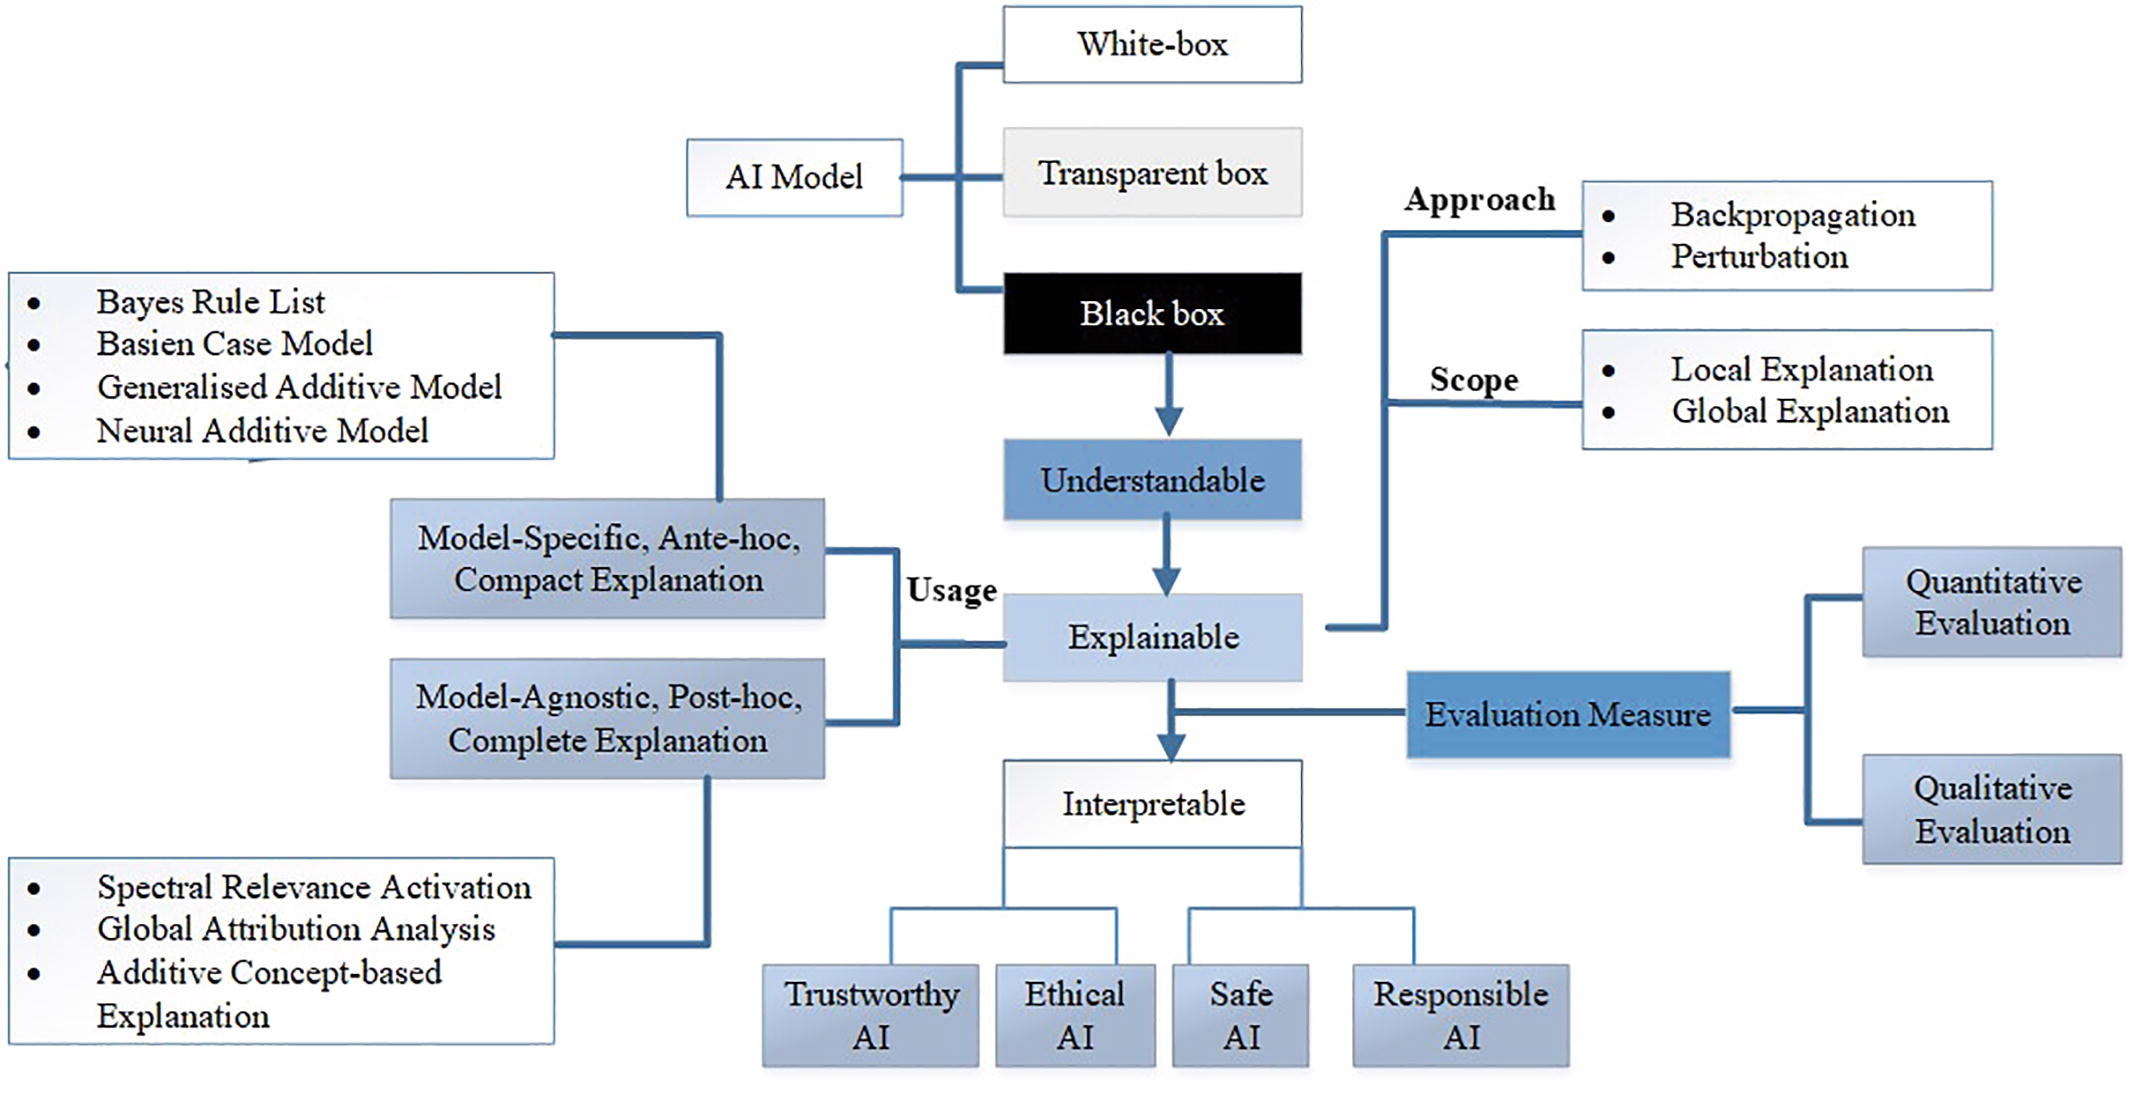
\includegraphics[width=0.7\textwidth]{images/CH02_algorithms_overview_Saleem.jpg}
    \caption*{Overview of the concepts related to Explainability algorithms.}
    \label{fig:Explainability_overview}
\end{figure}

The two most widely adapted local, model-agnostic, post-hoc methods are \textit{SHAP} (SHapley Additive exPlanations) \parencite{Lundberg2017} and \textit{LIME} (Local Interpretable Model-agnostic Explanations) \parencite{Ribeiro2016}.

\textbf{SHAP} is based upon the use of Shapley values used in coalitional game theory and aims to weight the importance of each feature to the result by game-theoretically distributing the value of the final prediction among all features being included \parencite{Molnar2023}.
The key features of SHAP are (based on \cite{Molnar2023})
\begin{itemize}
    \item \textbf{Additivity}: All feature contributions can be summed up in a linear way, benefitting understandability of the explanations.
    \item \textbf{Local Accuracy}: SHAP values are locally accurate, as predictions for a given input can be calculated as a result of the expected model output and the specific score for the local input.
    \item \textbf{Missingness}: As missingness in features is attributed zero values, missingness does not skew outcomes.
    \item \textbf{Consistency}: SHAP values do not change upon model change, but only when the actual feature contributions change.
\end{itemize}

\textbf{LIME} is based upon trying to approximate the model's decision boundary locally by perturbing the input data and observing the change in the model's output \parencite{Molnar2023}.

A way of globally assessing model Explainability is the use of \textbf{(Global) Surrogate Models} (as opposed to e.g. the LIME algorithm, which can be considered a local surrogate model). 
These aim to make black-box algorithm decisions explainable by implementing white-box models to learn the decision criteria that the black-box model has established by being trained on the black-box predictions (compare e.g. \cite{Karim2023}).
Instead of making the predictions themselves explainable, these models aim to making the underlying decision criteria understandable \parencite{Molnar2023}.

\subsection{Explainability and Fairness}\label{subsec:Explainability_fairness}

In order to conclude this literature review, this section will evaluate how the the concepts of Fairness and Explainability are related to each other, showing that the analysis of each adds separate value to this thesis.

Explainability and Fairness within the field of Machine Learning do not inherently share the same scope. On the one hand, as an example, Explainability is a rather objective concept, focusing on describing a model's inner workings neutrally. 
Comparing that to Fairness it becomes apparent that the latter is a more subjective concept, as it is dependent on the context and man-made definitions, which are often rooted in certain (e.g.\ political) interpretations of Fairness \parencite{Deepak2021}.
Yet, both concepts are somewhat dependent as assessing model fairness requires an understanding of the factors influencing a prediction \parencite{Zhou2022}.
Subsequently, approaches to connect both concepts have been proposed in academic literature. 
%Two different approaches are proposed by Deepak \parencite{Deepak2021}: 
%\begin{itemize}
%    \item \textbf{Interpretability for Fairness (IFF)}: IFF is a framework intending to ensure that supposedly fair decisions made by AI are truly fair. The two steps in order to achieve that are \textit{clearly laying out the values supposed to adhered to} and \textit{explaining decisions made with regards to how they relate to those values}.
%    \item \textbf{Fairness and Interpretations (F\&I)}: F\&I is a multi-layered approach, which, in the first step, aims to satisfy both Fairness and Interpretability requirements based on given constraints. If both criteria in combination cannot satisfyingly be met, the user needs to be informed that the model is not sufficiently interpretable, but yet adheres to at least one of the two desired properties.
%\end{itemize}
However, these concepts are only stated on theoretical level without practical implications in this paper and are therefore not directly applicable for practitioners.


% Following Zhou's line of reasoning \parencite{Zhou2022}, other important approaches to merge the ideas of Fairness and Explainability in academic literature include:

% \textbf{Explanation as a way of guaranteeing Fairness}: ... Papers!

% \textbf{Explanation as a way of shaping the perception of Fairness}: ... Papers!

% \textbf{Perceived Fairness of feature properties}: ... Papers!


Another promising approach to merge the concepts of Fairness and Explainability is the identification of root-causes for a certain model behavior by identifying \textit{influential subsets} within the underlying datasets as proposed by Pradhan \parencite{Pradhan2022}\footnote{For additional information on the proposed model see https://github.com/romilapradhan/gopher}.
By combining Explainability criteria ('Why is a certain subgroup influential on the model's outcome?') with Fairness criteria ('In how far can intervention in the training data regarding these subsets improve Fairness?'), the authors manage to implement an efficient algorithm combining both concepts.

%To-Do:
%Go through sources of Zhou and list important ones
%Mention specifically newly added analysis in this thesis
%Circle back to introduction: Why do both add value?

This thesis will add value to the discussion of Fairness and Explainability in Machine Learning by providing a novel approach to the analysis of both concepts in the field of mortgage lending: 
By using explainability algorithms and enrichment data, the analysis of fairness will be supported and iteratively adjusted with the aim of finding the optimal balance of both concepts.